\UseRawInputEncoding
\documentclass[12pt,letterpaper]{article}

\usepackage{times}
\usepackage[utf8]{inputenc}
\usepackage{amsmath}
\usepackage{amsfonts}
\usepackage{amssymb}
\usepackage{graphicx}
\usepackage{multicol}
\usepackage{changepage}
\usepackage{float}
\usepackage{url}
\usepackage{hyperref}
\usepackage{afterpage}
\usepackage{hyperref}

\usepackage[left=2cm, right=2cm]{geometry}
\usepackage[spanish]{babel}

%\graphicspath{ {./Images/} }

\author{Nombre}
\title{Portada siempre practica}

\begin{document}

%encabezado
\pagestyle{plain}{
\pagestyle{empty}
\changepage{3cm}{1cm}{-0.5cm}{-0.5cm}{}{-2cm}{}{}{}
\noindent

%sEGIUN EL formato de sus imagenes, deben encontrar una configuracion adeacuada para ustedes
{\small
\begin{tabular}{p{0.626\textwidth} p{0.50\textwidth} }

\end{tabular}
}

%datos de la caratula
\begin{center}
\par\vspace{1cm} %Espacio dejado antes del encabezado
{
\Huge\textbf{Hilos}
}
\par\vspace{5cm}
{
\Large{Juan Camilo Arteaga Ibarra}
}
\par\vspace{3cm}
{
\large{Tutor \\Augusto Enrique Salazar Jim\'enez } 
}
\par\vspace{4cm}
{
\large{Universidad de Antioquia \\Facultad de Ingenier\'ia }
}
\par\vspace{2cm}
{
\large{Inform\'atica 2}
}
\par\vspace{1cm}
{
\large{2019 - 2}
}
\end{center}
\clearpage
}
\setlength{\parindent}{0cm}
\normalsize
El flujo de control de las tareas de un microprocesador son administradas por una unidad básica llamada hilo, este se encarga de dividir en dos o más tareas (subprocesos), que pueden ser simultáneas o seudo simultáneas, a un programa que está en ejecución. Cada subproceso se asigna a una de estas unidades lógicas denominadas como hilos, existentes debido a la programación de la unidad de control. Una vez asignadas, las divisiones de la tarea principal se alternan en ejecución de modo en que aparenta realizarse dos o más procesos al mismo tiempo, permitiendo lograr un control eficaz en el tiempo de espera de los procesos y el ahorro de recursos, una optimización del funcionamiento de un microprocesador \cite{Threading}. \\[0.5cm]

\begin{figure}[h]
    \centering
    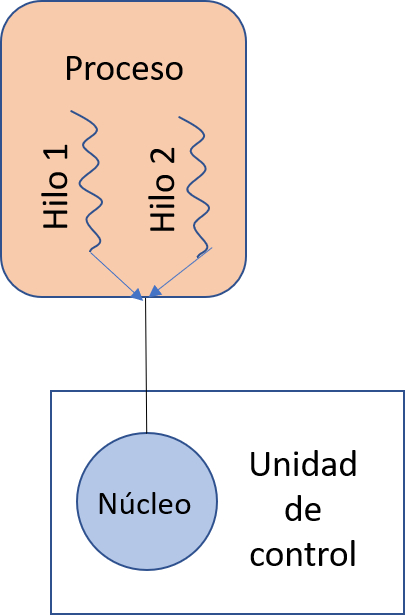
\includegraphics[width=6cm, height=8cm]{Threads.png}
    \caption{\label{Figura 1} gráfico funcionamiento.}
\end{figure} 

El origen de los hilos no es muy exacto, se tiene una noción de su aparición a mediados del año 1965, con el diseño del OS/360 de IBM mencionada en los comentarios de Dijkstra \cite{Dijkstra}. El lenguaje PL/I definido por IBM realizaba procesos pesados, tareas que dieron como resultado un hilo, pero se cree que nunca fue implementado debido a falta de protección entre de los hilos de control. Años más tarde en 1970 Max Smith hizo un prototipo en donde utilizaba múltiples ``stacks'' en un proceso pesado para poder aguantar compilaciones en segundo plano. Alrededor de la década de los setentas llegó Unix, que permitiendo la realización de procesos con máquinas pesadas, las cuales no podían compartir memoria. Al ver este problema se crearon los hilos, subprocesos que compartían las direcciones de memoria de un único proceso de Unix, dando entrada a los primero micro-núcleos. Se cree que gracias a estos acontecimientos se pudo continuar mejorando los ``subprocesos'' hasta consolidar la idea de lo que es son los hilos. Pero es importante mencionar que no se tienen datos certeros sobre la utilización de estos métodos para la realización de las tareas de un procesador \cite{History}. \\[1.5cm]

Hay dos tipos de hilos \cite{THilos}: 
\begin{itemize}
    \item \textbf{A nivel de usuario (ULT):} la aplicación es quien se encarga de la gestión de los hilos, por lo que para estos no es necesario que el SO ayude en el proceso. Para poder programar estos hilos es necesario hacer uso de alguna librería de hilos. Gracias a estos hilos el usuario tiene permitido realizar planificaciones específicas de ejecución. 
    \item \textbf{A nivel de kernel o núcleo (KLT):} todo el trabajo es realizado por el núcleo, los crea y los organiza para las tareas a ejecutar. Gracias a este tipo de hilos los procesos se realizan mucho más rápido y se ahorran recursos.\\[0.5cm]
\end{itemize}

Estos hilos a nivel de usuario y de kernel tienen tres relaciones \cite{THilos}, que son:
\begin{itemize}
    \item \textbf{One to one:} cada hilo del usuario se asigna a uno del kernel.
    \item \textbf{Many to one:} varios hilos de usuario se asignan a uno del kernel. Son hilos a nivel de usuario.
    \item \textbf{Many to many:} Un número de hilos de usuario se asignan a una igual o menor cantidad de hilos del kernel.\\[0.5cm]
\end{itemize}

\begin{figure}[h!]
    \centering
    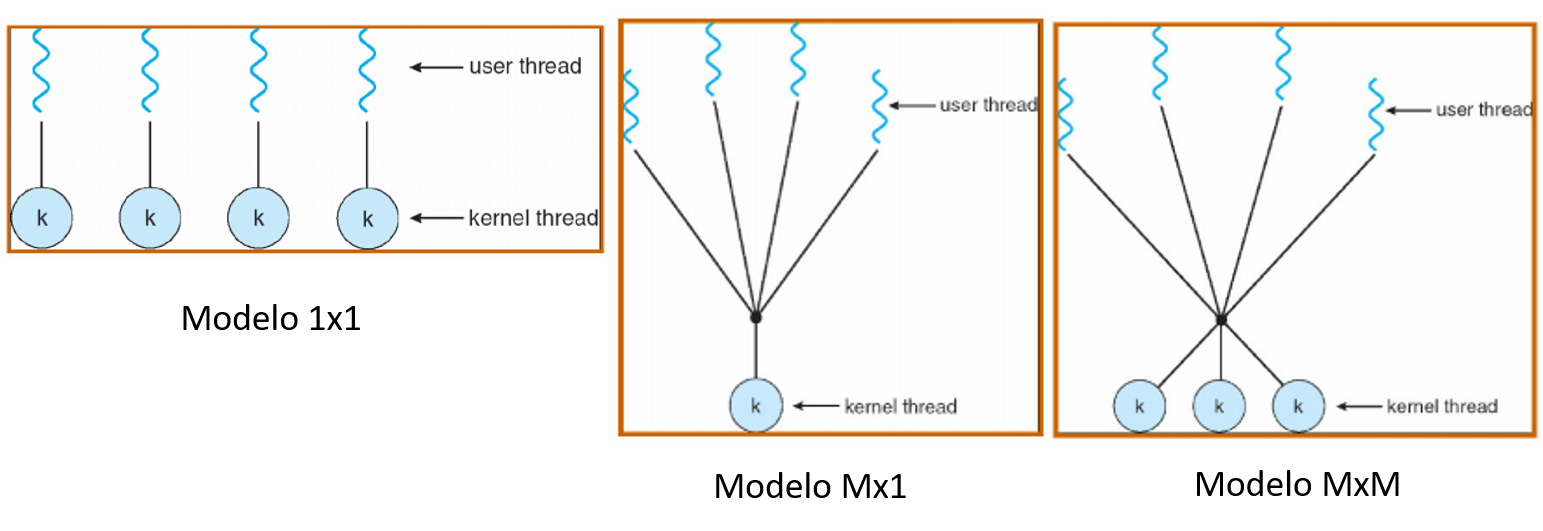
\includegraphics[width=18cm, height=7cm]{Modelos.png}
    \caption{\label{Figura 2} Pg 2, 3 \cite{THilos}}
\end{figure} 

Un procesador y/o un microprocesador pueden tener un solo hilo o varios hilos. Si la unidad de control solo tiene un hilo (single-threading) entonces solo procesa un comando a la vez, pero si tiene varios hilos entonces puede hacer que una tarea se divida en subprocesos que pueden ser ejecutados simultáneamente o muy a la par. El tener más de un hilo permite que haya una respuesta rápida a problemas, una ejecución más rápida, un menor consumo de recursos, un mejor uso del sistema y una forma más eficaz de comunicación interna \cite{Hilos}. \\[1cm]

Actualmente existen dos implementaciones de los hilos, a nivel de hardware y a nivel de software. 
\begin{itemize}
    \item En cuanto a la implementación de los hilos a nivel de hardware es la que viene por defecto en el microprocesador o el procesador, la estos poseen una cantidad de núcleos e hilos que pueden utilizar para la realización de procesos, los hilos que posee la unidad de control son reconocidos por el kernel, es decir, son hilos a nivel de kernel, lo que quiere decir que son limitados, dependen del hardware, por ejemplo si de fábrica se establece que tenga ocho hilos no puede poseer un número mayor de hilos a ocho, pero si puede dejar de utilizar un número menor al establecido de fábrica al momento de realizar la ejecución de un proceso \cite{quora}.
    \item Por otro lado la implementación a nivel de software, hilos a nivel de usuario, se pueden tener tantos hilos como se deseen, pero hay que atender a la relación que se esté haciendo con los que están a nivel del kernel. En la relación uno a uno hay una limitación de cuántos hilos implementados en el software se pueden tener, dependería del hardware que se tenga. Otra cosa a tener en cuenta con los hilos implementados a nivel de software es el lenguaje en el que se están programando, la velocidad con la que se realicen los subprocesos de una tarea establecida dependerán de este, además, algunas funciones para el uso de estos hilos dependen de las librerías diseñadas para la creación de los mismos, por tanto algunos lenguajes pueden tener limitadores en las funciones que tienen los hilos \cite{stack}.
\end{itemize}


\newpage
\renewcommand\refname{Referencias}
%\bibliographystyle{abntex2-alf}
\bibliographystyle{IEEEtran}
\bibliography{bibliography.bib}
%\listoftodos
\end{document}
